%\vspace{1.5pc}
\vspace{1.5pc}
%\section[State of the Art]{State of the Art}
\vspace{-1pc}
\section[Penelitian Terkait dan Tahapan Penelitian IOD]{Penelitian Terkait dan Tahapan Penelitian IOD}
\begin{spacing}{1.5}
	Hasil analisis data observasi selama 40 tahun (1958-1997) menunjukkan fenomena mode dipol di Samudera Hindia. Pola variasi internal dengan anomali \textit{sea surface temperature} (SST) rendah di sekitar Sumatra dan tinggi di sebelah barat Samudera Hindia, disertai dengan angin dan presipitasi. Keterkaitan spasial-temporal antara SST dan angin kuat melalui medan presipitasi dan dinamika laut. Proses interaksi udara-laut ini unik dan terbukti independen dari fenomena Osilasi Selatan El Nino (ENSO). Penemuan mode dipol ini menjelaskan sekitar 12\% variasi SST di Samudera Hindia, yang juga menyebabkan curah hujan yang parah di Afrika Timur dan kekeringan di Indonesia selama tahun-tahun aktifnya \cite{Saji1999}.
	
	\citeA{Liu2023} menunjukkan anomali salinitas positif yang signifikan di lapisan atas Samudera Hindia tropis pusat selama periode tertentu. Pada tahun 2010 dan 2016, pengaruh La Nina dan IOD negatif (nIOD) menyebabkan anomali salinitas positif di Samudera Hindia timur akibat adanya angin barat yang kuat dan arus zona positif. \citeA{Chu2022} mempelajari dinamika variasi antartahunan arus khatulistiwa di Samudera Hindia dan mengukur efek dari mode iklim ENSO dan IOD pada arus. \citeA{Xing2022} mengeksplorasi respons arus laut khatulistiwa selama fase puncak IOD, yang memberikan umpan balik positif laut yang mendukung puncak IOD. \citeA{Zhang2021} meneliti tentang Atlantic Nino dan dampaknya pada iklim regional dan global. Mereka menemukan bahwa curah hujan yang meningkat di sebelah barat Samudra Hindia tropis selama IOD positif (pIOD) melemahkan pertukaran angin timur di atas Samudra Atlantik tropis, menyebabkan anomali hangat di wilayah pusat dan timur khatulistiwa Atlantik sehingga memicu Atlantik Nino.
	
	\citeA{Polonsky2021} mengkaji fitur pembentukan lapisan kritis di zona ekuator-tropika Samudera Hindia, dan bagaimana hal tersebut terkait dengan terbentuknya IOD. \citeA{Valsala2020} meneliti dampak IOD pada siklus karbon di atas laut dan variasinya di Samudera Hindia, dengan menggunakan pengamatan biogeo kimia dan model sirkulasi biogeo kimia laut global. Mereka menemukan bahwa IOD menyebabkan variasi signifikan dalam pengeluaran CO$_2$ dari laut ke udara di wilayah tenggara tropika Samudera Hindia karena dinamika \textit{upwelling} dan anomali bergerak ke barat. \citeA{Zhang2020} membedakan IOD dari pola tripole baru yang baru saja ditemukan, yang memiliki \textit{sea surface temperature anomalies} (SSTA) positif (negatif) di atas wilayah tengah tropika (tenggara dan barat) Samudera Hindia. Studi-studi ini membantu untuk memahami interaksi kompleks antara arus laut, kondisi atmosfer, dan variabilitas iklim di Samudera Hindia.
	
	Terkait dengan SST dan \textit{sea surface salinity} (SSS), \citeA{Akhil2023} menemukan bahwa penyegaran permukaan laut di bagian tenggara Laut Arab (SEAS) selama musim dingin dipicu oleh adveksi horizontal air tawar \textit{Bay of Bengal} (BoB) oleh sirkulasi siklonik di sekitar India selama musim gugur, dan IOD menjadi penggerak utama dari variasi antartahunan SSS di SEAS selama musim dingin. Namun, dampak penyegaran SEAS musim dingin terhadap SST lokal dan awal musim hujan berikutnya lemah. Studi lain oleh \citeA{Genda2022} menemukan bahwa sebelum pertengahan 1950-an, SST bervariasi dengan IOD, sedangkan ENSO juga mempengaruhi variasi SST setelah pertengahan 1950-an. Variasi SSS tidak menunjukkan hubungan dengan faktor-faktor iklim, mengindikasikan bahwa faktor-faktor pengontrol utama SST dan SSS harus dipertimbangkan secara terpisah. Selain itu, \citeA{Sun2022} meneliti respons asimetris SSS yang signifikan terhadap dua kejadian pIOD dan nIOD di Selatan Samudera Hindia tropis. Beberapa studi lain juga menyoroti pentingnya IOD dalam menggerakkan variasi antartahunan SSS, seperti penelitian oleh \citeA{Rathore2020} yang menggunakan komposit musiman selama peristiwa ENSO/IOD untuk memahami variasi dalam transportasi kelembaban dan curah hujan di atas Australia, serta asosiasi mereka dengan variasi SSS. Studi lainnya oleh \citeA{Sun2019} dan \citeA{Zhang2016} mengidentifikasi mode dipol salinitas di Samudera Hindia tropis, yang disebut S-IOD, pola variasi SSS antar tahunan dengan anomali salinitas rendah di bagian tengah khatulistiwa dan salinitas tinggi di sebelah tenggara Samudera Hindia tropis.
	
	Selain itu, terdapat penelitian tentang dampak IOD pada kedalaman lapisan campuran (MLD) di Samudera Hindia, seperti penelitian oleh \citeA{Sadhukhan2021} yang menemukan bahwa peristiwa nIOD berasosiasi dengan MLD yang lebih dalam di BoB sedangkan pIOD menyebabkan MLD yang lebih dangkal. Korelasi parsial menunjukkan bahwa fluks panas bersih (NHF) adalah kontributor utama pendalaman MLD di atas BoB utara, sedangkan tekanan angin mengontrol pendalaman di atas BoB selatan. \citeA{Zhang2022} menunjukkan bahwa selama nIOD, MLD menurun karena daerah anomali evaporasi minus presipitasi negatif. Sebaliknya, selama pIOD, MLD meningkat karena daerah anomali evaporasi minus presipitasi positif. 
	
	\citeA{Sun2019} menyelidiki variasi SSS dan hubungannya dengan dinamika laut di Samudera Hindia tropis selatan barat (SWTIO) terkait dengan peristiwa IOD negatif tahun 2010. Mereka menemukan bahwa sirkulasi laut di Samudera Hindia selatan tropis berkontribusi secara signifikan terhadap anomali SSS selama evolusi peristiwa IOD negatif. Kenaikan gelombang Rossby membuat kedalaman termoklin dan MLD dangkal, membawa air subpermukaan berkepadatan tinggi ke lapisan permukaan dan mendinginkan SST, yang lebih menekan presipitasi lokal untuk memberikan umpan balik positif bagi peningkatan SSS. \citeA{Dandapat2021} menemukan bahwa MLD dangkal selama pIOD pada tahun 2006, sedangkan MLD rata-rata lebih dalam (sekitar 50 m) selama nIOD pada tahun 2010. Fluks panas bersih positif pada antarmuka udara-laut juga memainkan peran dominan dalam pendangkalan MLD pada tahun pIOD, karena radiasi gelombang pendek meningkat dan melebihi efek pendinginan fluks panas laten selama periode ini. 
	
	\citeA{Sari2020} menemukan bahwa selama peristiwa IOD positif kanonik, konsentrasi chl-a yang tinggi diamati di sekitar Selat Sunda dan sepanjang pantai ujung barat Pulau Jawa di sekitar wilayah Cilacap. Sementara itu, selama peristiwa IOD positif Modoki, konsentrasi chl-a yang relatif lebih tinggi dan lebih terdistribusi luas daripada yang diamati selama peristiwa IOD positif kanonik. Analisis menunjukkan bahwa peristiwa upwelling yang relatif lemah yang ditunjukkan oleh kedalaman lapisan isotermal yang dalam (ILD) selama peristiwa IOD positif Modoki yang dikombinasikan dengan ketebalan lapisan penghalang yang tipis (BLT) dan lapisan campuran yang dalam memberikan kondisi yang menguntungkan untuk peningkatan konsentrasi chl-a di wilayah Southeastern Tropical Indian Ocean (SETIO). Sementara itu, upwelling yang kuat yang ditunjukkan oleh kedalaman ILD yang dangkal yang dikombinasikan dengan BLT yang tebal dan lapisan campuran yang dangkal mencegah peningkatan konsentrasi chl-a selama peristiwa IOD positif kanonik. Di sisi lain, \citeA{Devi2017} menemukan bahwa IOD positif menyebabkan konsentrasi chl-a yang rendah (<2 mg/m$^3$) dan produktivitas primer yang rendah di Laut Arab (AS). \citeA{Mandal2022} dan \citeA{Simanjuntak2022} membahas pengaruh ENSO dan IOD pada variasi chl-a, sementara \citeA{Luang-on2022} memfokuskan pada variasi musiman dan antar tahun konsentrasi chl-a di Teluk Thailand bagian atas. \citeA{Setiawan2020} menyelidiki hubungan antara konsentrasi chl-a, SST, dan tekanan angin permukaan laut di Laut Halmahera yang dipengaruhi oleh Monsun Australia-Indonesia (AIM), ENSO, dan IOD.
	
	
\end{spacing}
\vspace{-1pc}
\section[Model Numerik dan Parameter]{Model Numerik dan Parameter}
\begin{spacing}{1.5}
	\par Dalam subbab ini, akan dibahas mengenai persamaan untuk parameter dan deskripsi tentang model numerik yang digunakan dalam penelitian ini.
	
	Model sirkulasi laut atau \textit{Ocean General Circulation Models} (OGCM) menggunakan persamaan Navier-Stokes untuk memodelkan fenomena fisis yang terjadi di lautan. Lautan adalah fluida yang dapat dijelaskan dengan baik dengan pendekatan persamaan-persamaan primitif, yaitu persamaan Navier-Stokes serta persamaan keadaan nonlinier yang menggabungkan dua parameter (temperatur dan salinitas) dengan kecepatan fluida, dan mempertimbangkan beberapa asumsi dan hipotesis \shortcite{madec_gurvan_2022_6334656}.
	
	Beberapa asumsi yang digunakan dalam persamaan Navier-Stokes diantaranya asumsi Boussinesq, asumsi hidrostatik, dan asumsi tak termampatkan (\textit{incompressibility}). Misalkan $\rho$ sebagai densitas in situ, $T$ sebagai temperatur potensial, $S$ sebagai salinitas, $p$ sebagai tekanan, $z$ sebagai koordinat vertikal, dan $g$ sebagai percepatan gravitasi. Asumsi yang digunakan dalam persamaan Navier-Stokes dapat dituliskan sebagai berikut.\\
	Asumsi Boussinesq
	\begin{equation}\label{eq:P1}
		\rho = \rho(T,S,p).
	\end{equation}
	Berdasarkan asumsi Boussinesq, pengaruh variasi densitas terhadap sistem diabaikan kecuali kontribusinya terhadap gaya apung.\\
	Asumsi hidrostatik
	\begin{equation}
		\frac{\partial p}{\partial z} = -\rho g.
	\end{equation}
	Berdasarkan asumsi hidrostatik, persamaan momentum vertikal direduksi menjadi persamaan kesetimbangan antara parameter gradien tekanan vertikal dan gaya apung.\\
	Asumsi tak termampatkan
	\begin{equation}
		\nabla \;.\; U =\frac{\partial u}{\partial x} + \frac{\partial v}{\partial y} + \frac{\partial w}{\partial z} = 0.
	\end{equation}	
	Berdasarkan asumsi tak termampatkan, persamaan 3-D divergensi untuk vektor kecepatan $U = (u,v,w)$ (dalam koordinat kartesius $(x,y,z)$) dianggap sama dengan 0.
	
	Selanjutnya misalkan $U = U_h + wk$ ($h$ adalah notasi vektor horizontal lokal di atas bidang $(i,j)$). Persamaan vektor invarian (invarian di bawah transformasi koordinat sehingga dapat diterapkan secara seragam dalam sistem koordinat lengkung ortogonal mana pun) dari persamaan primitif dalam sistem vektor $(i, j, k)$ dapat dituliskan dalam persamaan berikut \shortcite{madec_gurvan_2022_6334656}.\\
	Persamaan kesetimbangan momentum
	\begin{equation}\label{eq:P2}
		\begin{aligned}
			\frac{\partial U_h}{\partial t} = - \left[(\nabla \times U) \times U + \frac{1}{2}\nabla (U^2)\right]_h - f \; k \times U_h - \frac{1}{\rho_o}\nabla_h p + D^U + F^U.
		\end{aligned}
	\end{equation}
	Dalam Persamaan (\ref{eq:P2}) di atas, suku $(\nabla \times U) \times U + \frac{1}{2}\nabla (U^2)$ dapat ditulis sebagai $U\cdot \nabla U$ dan merupakan suku percepatan konvektif dari persamaan momentum. Suku $\nabla_h p$ merupakan gradien tekanan, $f = 2\Omega\; \cdot \;k$ merupakan percepatan Coriolis (dengan $\Omega$ adalah vector kecepatan sudut bumi), $D^U$ merupakan parameterisasi dari fisika skala kecil untuk momentum sedangkan $F^U$ merupakan suku gaya permukaan untuk momentum.\\
	Persamaan konservasi panas dan salinitas
	\begin{equation}\label{eq:P3}
		\begin{aligned}
			\frac{\partial T}{\partial t} &= - \nabla \; . \; (T\;U)  + D^T + F^T \\
			\frac{\partial S}{\partial t} &= - \nabla \; . \; (S\;U)  + D^S + F^S,
		\end{aligned}
	\end{equation}
	dengan operator $\nabla$ sebagai vektor turunan yang diperumum dalam arah $(i,j,k)$, parameter $D^T$ dan $D^S$ merupakan parameterisasi dari fisika skala kecil untuk temperatur dan salinitas sedangkan parameter $F^T$ dan $F^S$ merupakan suku gaya permukaan untuk temperatur dan salinitas. 
	
	Untuk parameter lainnya seperti kedalaman lapisan campuran atau \textit{mixed layer depth} (MLD), \textit{chlorophyll-a} (Chl-a), laju presipitasi, fluks air tawar, fluks panas bersih, dan tekanan angin dapat dituliskan sebagai berikut.
	
%	Dalam aplikasinya, persamaan Navier-Stokes tidak hanya digunakan untuk memodelkan laut, tapi juga merambah ke bidang pemodelan cuaca \shortcite{Rohli2021}, aliran air dalam pipa \shortcite{Ouchiha2012} dan aliran udara di sekitar sayap pesawat \shortcite{Tulus2019}. Dalam bentuk persamaan lengkap dan simplifikasi, persamaan ini juga dapat digunakan untuk mendesain kereta api \shortcite{Croquer2020}, pesawat terbang \shortcite{Chau2021}, dan mobil \shortcite{Ambarita2018}. Terdapat juga studi tentang aliran darah \shortcite{Gill2021}, desain stasiun pembangkit listrik \shortcite{Yang2019}, dan analisis polusi udara \shortcite{Issakhov2022}. 
	
\end{spacing}
\vspace{-1pc}
\section[\textit{Road Map }Penelitian]{\textit{Road Map} Penelitian}
\begin{spacing}{1.5}
	\textit{Road Map} penelitian ini dapat dilihat dalam Gambar \ref{fig:RM}
	\begin{figure}[H]
		\centering
		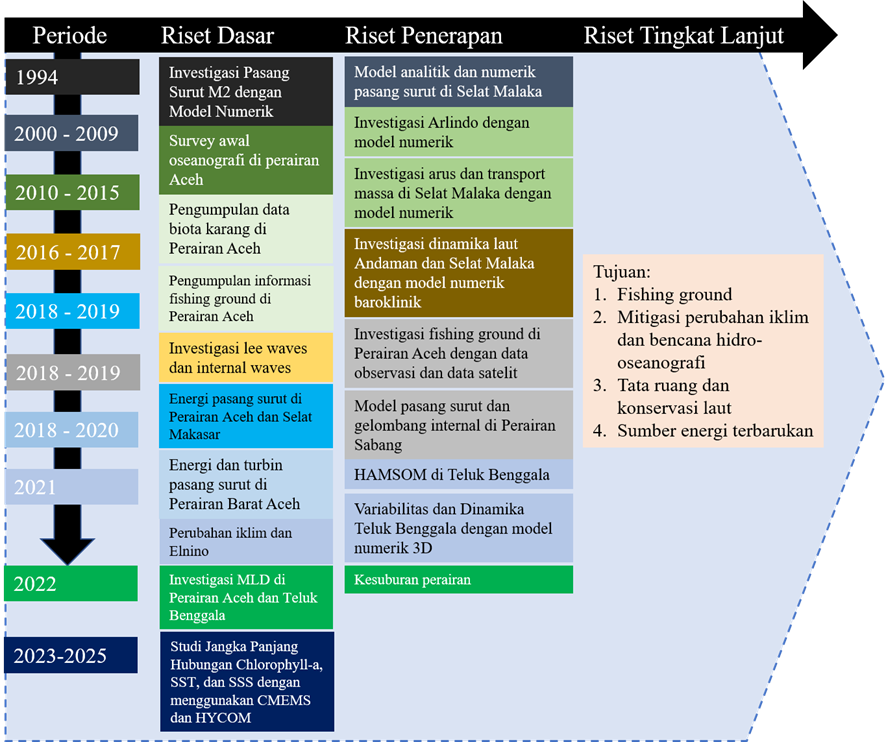
\includegraphics[width=12cm]{contents/Figures/Road_Map}
		\caption{Road Map Penelitian}
		\label{fig:RM}
	\end{figure}
	
\end{spacing}